% BSD 3-Clause License
%
% Copyright (c) 2023, 2024 Quux System and Technology. All rights reserved.
%
% Redistribution and use in source and binary forms, with or without
% modification, are permitted provided that the following conditions are met:
%
% 1. Redistributions of source code must retain the above copyright notice, this
%    list of conditions and the following disclaimer.
%
% 2. Redistributions in binary form must reproduce the above copyright notice,
%    this list of conditions and the following disclaimer in the documentation
%    and/or other materials provided with the distribution.
%
% 3. Neither the name of the copyright holder nor the names of its
%    contributors may be used to endorse or promote products derived from
%    this software without specific prior written permission.
%
% THIS SOFTWARE IS PROVIDED BY THE COPYRIGHT HOLDERS AND CONTRIBUTORS "AS IS"
% AND ANY EXPRESS OR IMPLIED WARRANTIES, INCLUDING, BUT NOT LIMITED TO, THE
% IMPLIED WARRANTIES OF MERCHANTABILITY AND FITNESS FOR A PARTICULAR PURPOSE ARE
% DISCLAIMED. IN NO EVENT SHALL THE COPYRIGHT HOLDER OR CONTRIBUTORS BE LIABLE
% FOR ANY DIRECT, INDIRECT, INCIDENTAL, SPECIAL, EXEMPLARY, OR CONSEQUENTIAL
% DAMAGES (INCLUDING, BUT NOT LIMITED TO, PROCUREMENT OF SUBSTITUTE GOODS OR
% SERVICES; LOSS OF USE, DATA, OR PROFITS; OR BUSINESS INTERRUPTION) HOWEVER
% CAUSED AND ON ANY THEORY OF LIABILITY, WHETHER IN CONTRACT, STRICT LIABILITY,
% OR TORT (INCLUDING NEGLIGENCE OR OTHERWISE) ARISING IN ANY WAY OUT OF THE USE
% OF THIS SOFTWARE, EVEN IF ADVISED OF THE POSSIBILITY OF SUCH DAMAGE.
%
\begin{recipe}{叉烧宣腿}

\ingredients

\ingredient{宣腿}{二斤}
\ingredient{荷叶饼}{十二个}
\ingredient{面包}{八两}
\ingredient{干豆粉}{三钱}
\ingredient{鸡蛋}{二个}

\preparation

\step 选用硬边宣腿一方,用温水洗净,用刀将附于火腿上的黑色薄皮刮尽。

\begin{wrapfigure}[13]{l}{11em}%
\centering%
\vspace{-.75\baselineskip}%
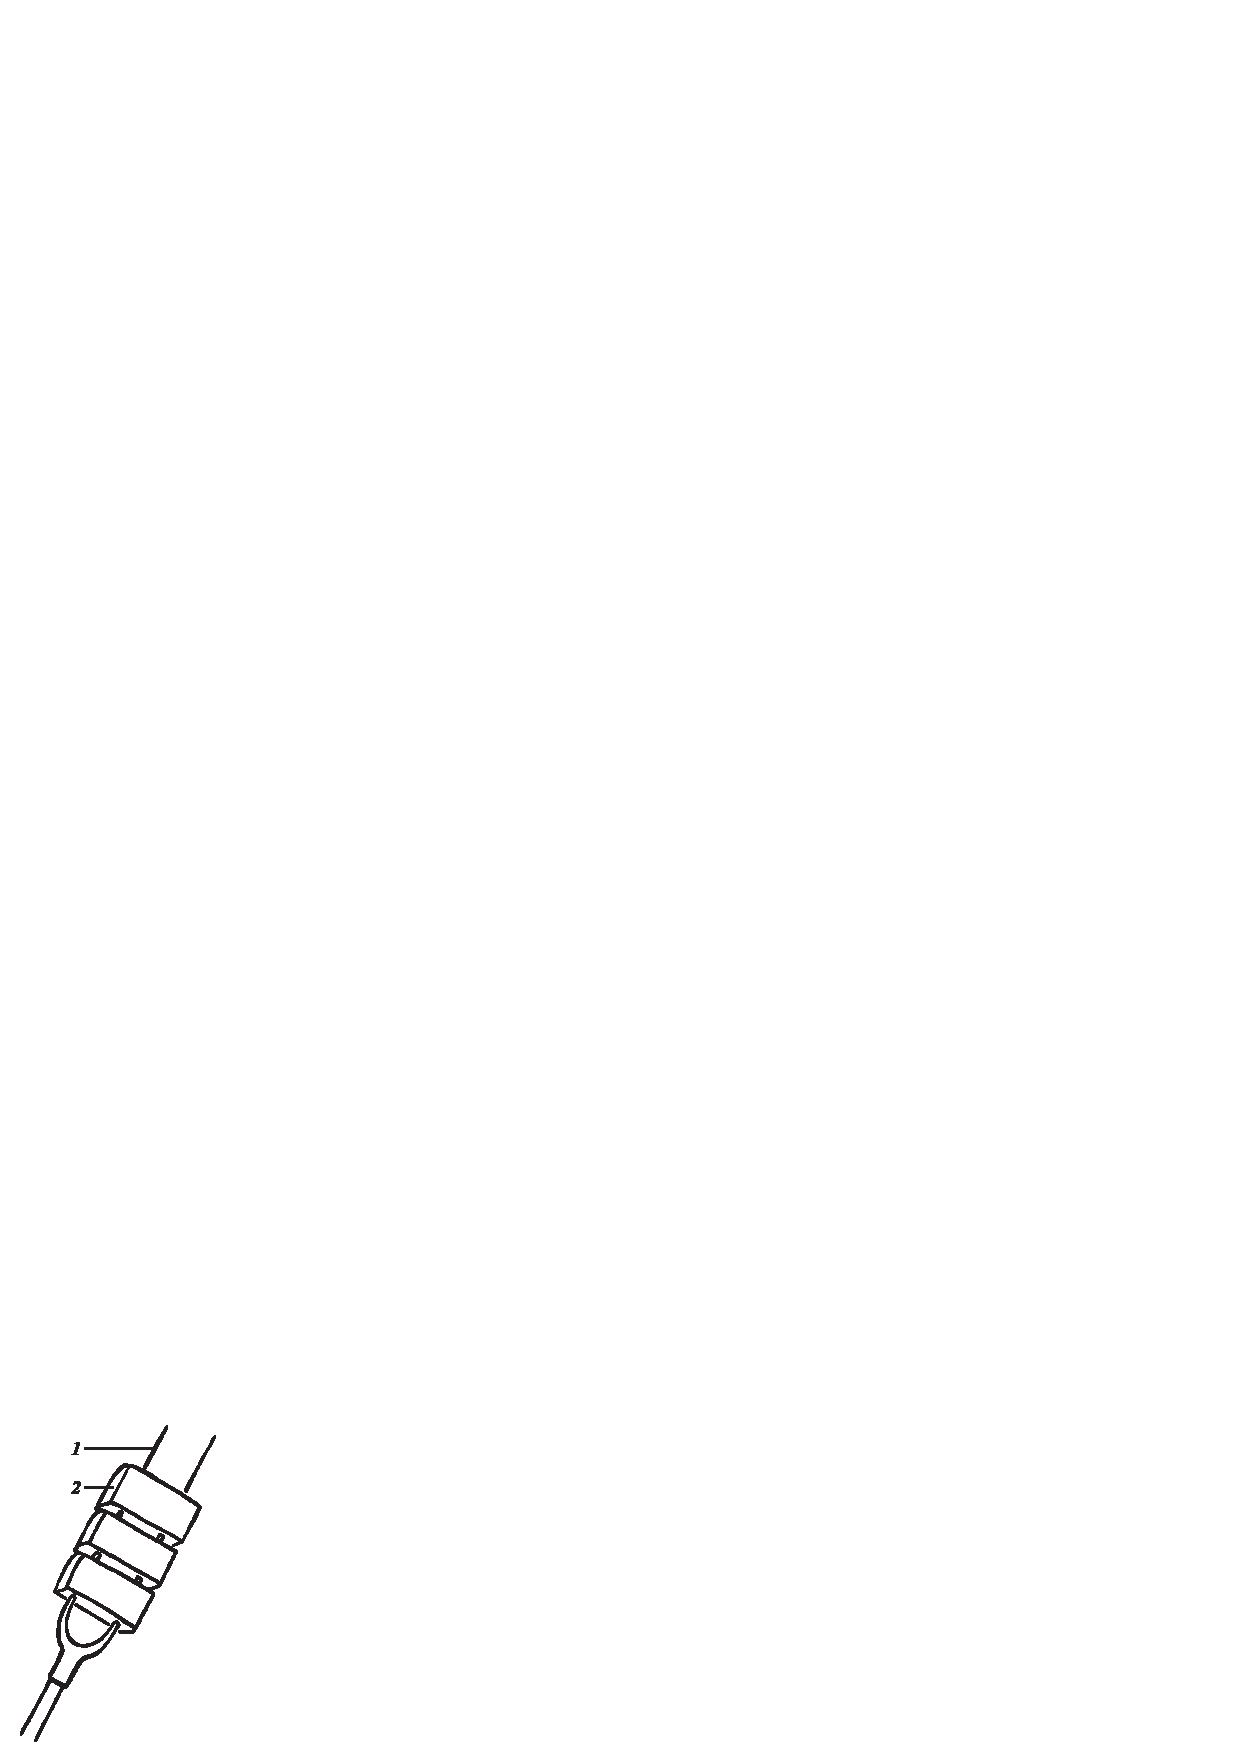
\includegraphics[scale=1]{illustration-011.pdf}%
\vspace{-.4375\baselineskip}%
\caption{叉烧宣腿叉法}
\label{fig:skewering-method}%
\begingroup%
\small%
\noindent%
\null\hspace{0em}1.铁叉\hspace{1em}2.火腿
\endgroup%
\end{wrapfigure}

\step 用刀将火腿均匀地切为三块,每块切成一寸三分宽、四寸半长,厚度为火腿本身的
厚度,用铁叉平叉起来(如图\,\ref{fig:skewering-method}\,)。将蛋清与豆粉调匀,
涂于叉起来的火腿上以保持原味,而免烧时走油走味。

\step 把杠炭三斤放入平炉上烧红,而后把叉好的火腿在平炉上以微火烘烤,要反复转动
叉柄,约二十分钟,烤至火腿熟透心时,揩净叉尖后取下叉子。用刀把火腿每隔两分远切
一刀,但不要完全切断,使其不会分开。然后摆在盘中,下面摆两块、上面摆一块成为
“品”字形。与烤熟的面包(切为十二片)和蒸好的荷叶饼同时上席。

\features

此菜外酥内香,为下酒的好菜。

\end{recipe}

% vim: filetype=tex noautoindent nojoinspaces
% vim: fileencoding=utf-8 formatoptions+=m
% vim: textwidth=78 tabstop=4 shiftwidth=4 softtabstop=4
